\documentclass{beamer}


\usetheme{Madrid}
\usepackage{graphicx} % Allows including images
\usepackage{booktabs} % Allows the use of \toprule, \midrule and \bottomrule in tables
\usepackage[czech]{babel}
%----------------------------------------------------------------------------------------
%	TITLE PAGE
%----------------------------------------------------------------------------------------

\title[amogus]{Historie počítačů} % The short title appears at the bottom of every slide, the full title is only on the title page

\author{Jáchym Löwenhöffer} % Your name
\institute[GEVO] % Your institution as it will appear on the bottom of every slide, may be shorthand to save space
{
Gynekologická Evaluace Velkých Obrazů \\ % Your institution for the title page
\medskip
\textit{jachym.lowenhoffer@gmail.com} % Your email address
}
\date{\today} % Date, can be changed to a custom date

\graphicspath{{./pics/}}

\AtBeginSection[]
{
  \begin{frame}
  \vfill
  \centering
  \begin{beamercolorbox}[sep=8pt,center,shadow=true,rounded=true]{title}
    \usebeamerfont{title}\insertsectionhead\par%
  \end{beamercolorbox}
  \vfill
  \end{frame}
}

\begin{document}

\begin{frame}
	\titlepage % Print the title page as the first slide
\end{frame}

\begin{frame}
	\frametitle{Přehled} % Table of contents slide, comment this block out to remove it
	\tableofcontents % Throughout your presentation, if you choose to use \section{} and \subsection{} commands, these will automatically be printed on this slide as an overview of your presentation
\end{frame}

%----------------------------------------------------------------------------------------
%	PRESENTATION SLIDES
%----------------------------------------------------------------------------------------
\section{Tuříngus}
\label{sec:turingus}


\begin{frame}
	\frametitle{Komp}
Abychom se mohli bavit o tom, co je počítač, musíme si ho definovat.
  \begin{block}{Definice počítače}
	 Provádí výpočty na určitých datech. Historicky nemusel být programovatelný,
	 ale teď již je tak často definovaný.
	\end{block}
	Podstata počítačů je aby lidem pomáhali se složitými výpočty. Tento účel
	plnili v minulosti například logaritmické tabulky, ovšem ty bychom z dnešního
	pohledu za počítače považovat nemohli.
\end{frame}

\begin{frame}
 \frametitle{Turingův stroj}
 Krom počítačů fyzických máme i počítačové modely, které slouží hlavně jako
 teoretické koncepty.

 \centering
 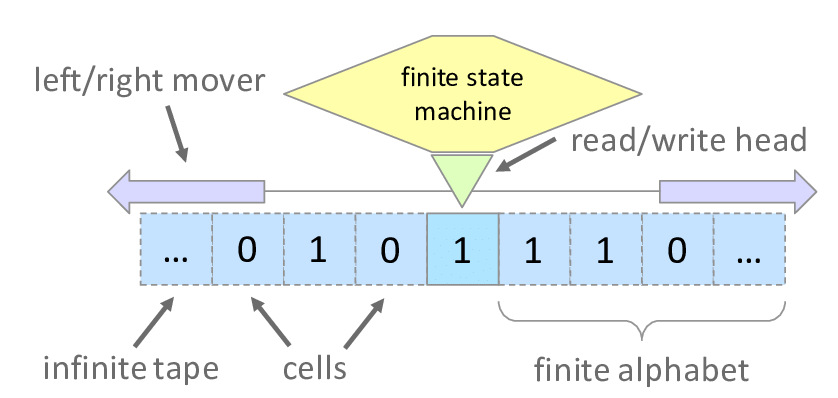
\includegraphics[scale=0.3]{turing.png}

\raggedright

 Turingův stroj je teoretický model s nekonečnou pamětí a jednoduchou hlavou,
 která buď čte, píše nebo se hýbe. To vše podle přechodové funkce.

 Podle tohoto modelu budeme hodnotit ostatní počítače.
\end{frame}

\begin{frame}
 \frametitle{Přechodová funkce}
 Slouží na rozhodnutí další akce Turignova stroje.

 Tato funkce má na vstupu:
 \begin{itemize}
  \item Aktuální stav stroje
  \item Hodnotu buňky na kterou ukazuje hlava
 \end{itemize}
 Podle předem naprogramovaných kritérií se poté rozhodne co dělat dál. Jeden z
 možných výstupů je změna stavu (nic tedy neděláme s hlavou jako takovou a
 spustíme tu samou funkci jen s jiným stavem na té stejné buňce).

 Můžeme zde vidět spojitost s Von Neumanovou architekturou a ta není vůbec
 náhodná. Konečný automat je dokonce součástí obou těchto modelů.
\end{frame}

\begin{frame}
 \frametitle{Podobnost Turinga s Neumanem}
 Hlavním rozdílem je že Turingův stroj má svojí přechodovou funkci uloženou
 úplně v jiné paměti než data na kterých operuje. 
 \vfill
 Druhým technickým detailem je, že Turingův stroj má ze základu slovo pouze o
 velikosti 1. To ale můžeme jednoduše změnit a donutit ho si do stavů zapisovat
 libovolně dlouhá slova.
\end{frame}

\begin{frame}
\frametitle{Byl Turing Turingovsky kompletní?}
Když už je řeč o Turignáčích, musíme si také uvést pojem Turingovsky kompletní.
\begin{block}{Turignovsky úplný}
nazveme instrukční sadu jestliže je schopna simulovat každou další Turingovsky
úplnou sadu. Někdy se také definuje jako schopnost instrukční sady simulovat
Turingův stroj. 
\end{block}
Abychom si tento termín předvedli uveďme si pár příkladů a protipříkladů.
\end{frame}

\begin{frame}
 \frametitle{Příklady}
 Začněme něčím co je triviálně Turingovsky kompletní: \textbf{python}. Jestliže chceme
 v pythonu simulovat Turingův stroj stačí nám pro to pár proměnných a poté
 přechodová funkce, kterou můžeme v pythonu napsat.

 Pozorného diváka by napadlo: vždyť python přeci nemůže mít nekonečnou paměť. A
 ano nemá; toto kritérium zpravidla vynecháváme.

 \vfill
 Teď opak. Každému asi došlo, že \textbf{logaritmické tabulky} nejsou turingovsky
 kompletní. Jestliže je budeme chtít převést na doslova jakýkoliv jiný program
 než ten co počítá logaritmy tak se nám to nepovede.
 
\end{frame}
\section{Předchůdci počítačů}
\label{sec:fde-cycle}

\begin{frame}
 \frametitle{Analogové a číslicové}
 \begin{block}{Analogové}
  Vstup berou veskrze spojitě a fungují na základě mechanických principů. Nejsou
  programovatelné a dají se tedy použít jen na velmi specifické úkoly.
 \end{block}

 \begin{block}{Číslicové}
  Tyto počítače jsou v principu ty co známe. Oproti analogovým berou vstup jako
  diskrétní sekvenci nul a jedniček (nebo jiných číslic počítáme-li úlety ze
  začátku počítačů). Fungují na fyzikálních principech a logických bránách.
  
 \end{block}

Historicky první byly ty analogové.
 \end{frame}



\section{Ve válce múzy mlčí}
\begin{frame}
 \frametitle{Ale vědci ne, get fucked kalkulačky jsou tady!!}
Cílem vývoje za druhé světové války bylo získat díky větší výpočetní síle
převahu. Němci i Američani měli vlastní prototypy, které byli velmi složité ale
již Turingovsky kompletní a občas i použitelné.\footnote{První kdo měl
teoretický model Turingovsky kompletního počítače byl Ch. Babbage v roce 1833}
\vfill
Input se stále musel zadávat ručně a jejich programování fungovalo přes děrné
štítky. Rychlost výpočetních instrukcí byla horší než jedna za sekundu.
\vfill
Tyto začátky počítačů ukazují jak je lidstvo ochotné důvěřovat technologii,
která ze začátku ničemu nepomáhá a svět ve kterém žijeme ukazuje jak se to čas
od času může vyplatit.
\end{frame}

\begin{frame}
 \frametitle{Omg rezistory}
 Během studené války se do počítačů začali dávat tranzistory které z nich
 udělali o hodně rychlejší, menší a efektivnější stroje. Začali se objevovat i v
 laboratořích kde pomáhali s výzkumem (například atomové bomby).
\vfill
 Byly vyvinuty nejprimitivnější operační systémy a pomalu se začínali vyrábět
 sériově.
\end{frame}
\begin{frame}
 \frametitle{Omg OS}
 S tím jak začali být počítače populární byla motivace je dělat co
 nejefektivnější a příjemné pro uživatele. Efektivita byla docíle tím, že
 počítač sám začal přepínat mezi svými úlohami aby na žádné z nich nečekal
 zbytečně.

 \vfill
 Za tímto účelem byly zdokonaleny operační systémy. Rozvoj OS pomáhá k rozvoji
 počítače jako technologie.
\end{frame}
\begin{frame}
 \frametitle{Je libo počítač do kapsy?}
 Dnes je počítač prakticky všude a z pravidla je připojený k internetu. Internet
 naplnil celý potenciál počítače jako technologie. Dá se říct, že poslední dobou
 tato technologie stagnuje.

 \vfill
To ale samozřejmě vedlo k vytvoření dalších technologií. Mezi ty nejzpytovanější
patří kvantové-počítače. Jako kuriozity zmiňme například počítače na bázi
fotonů.
\end{frame}

\end{document}
